\chapter{Klasifikacija}
\label{ch:klasifikacija}

Omenili smo že tip Aarne-Thompson (ATU)\marginnote{Aarne and Thompson sta folklorista, ki uvedla sistem klasifikacije ljudskih pravljic glede na podlagi motiva. Sistem je v uporabi od leta 1810 je pogosto v uporabi v primerjalni folkloristiki. Končna U v ATU pomeni Uther, ki je leta 2004 zadnji posodobil indeks.} To je indeks folklornih motivov in naše pravljice so že označene z visokonivojskim (žanr) in srednjenivojskim motivom (podžanr).

Ali bi morda lahko napovedali ATU tip na podlagi vsebine pravljice? Pa poglejmo.

\begin{figure}[h]
    \centering
    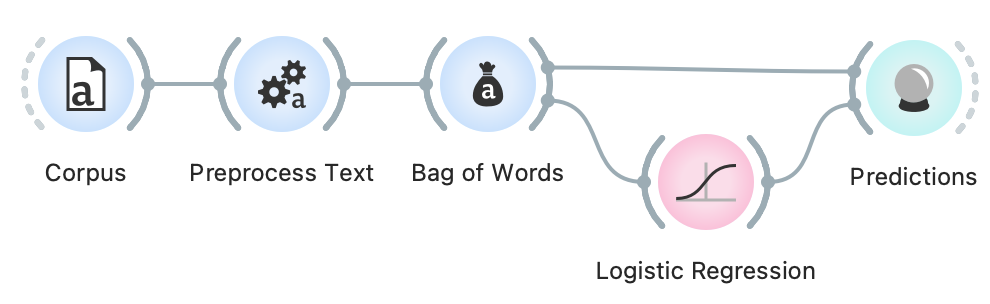
\includegraphics[width=0.9\linewidth]{klasifikacija-wf.png}%
    \caption{ }
    \label{fig:002-stop-words}
\end{figure}

Za začetek potrebujemo ciljno spremenljivko. To je spremenljivka, ki jo želimo napovedati, v našem primeru tip ATU. Potrebujemo tudi številsko reprezentacijo besedila - vrečo besed, ki nam jo je izračunal gradnik Bag of Word.

Sedaj bomo zgradili napovedni model. Model na podlagi enot (besed) napove ciljno vrednost (tip ATU). Vsak model potrebuje tudi postopek, ki definira, kako model upošteva besede. V našem primeru bo to logistična regresija.

V gradniku Predictions vidimo stolpec, kjer so napovedane vrednosti po postopku logistične regresije. Izgleda, da je naš model pravilno napovedal večino pravljic.

\begin{figure*}[h]
    \centering
    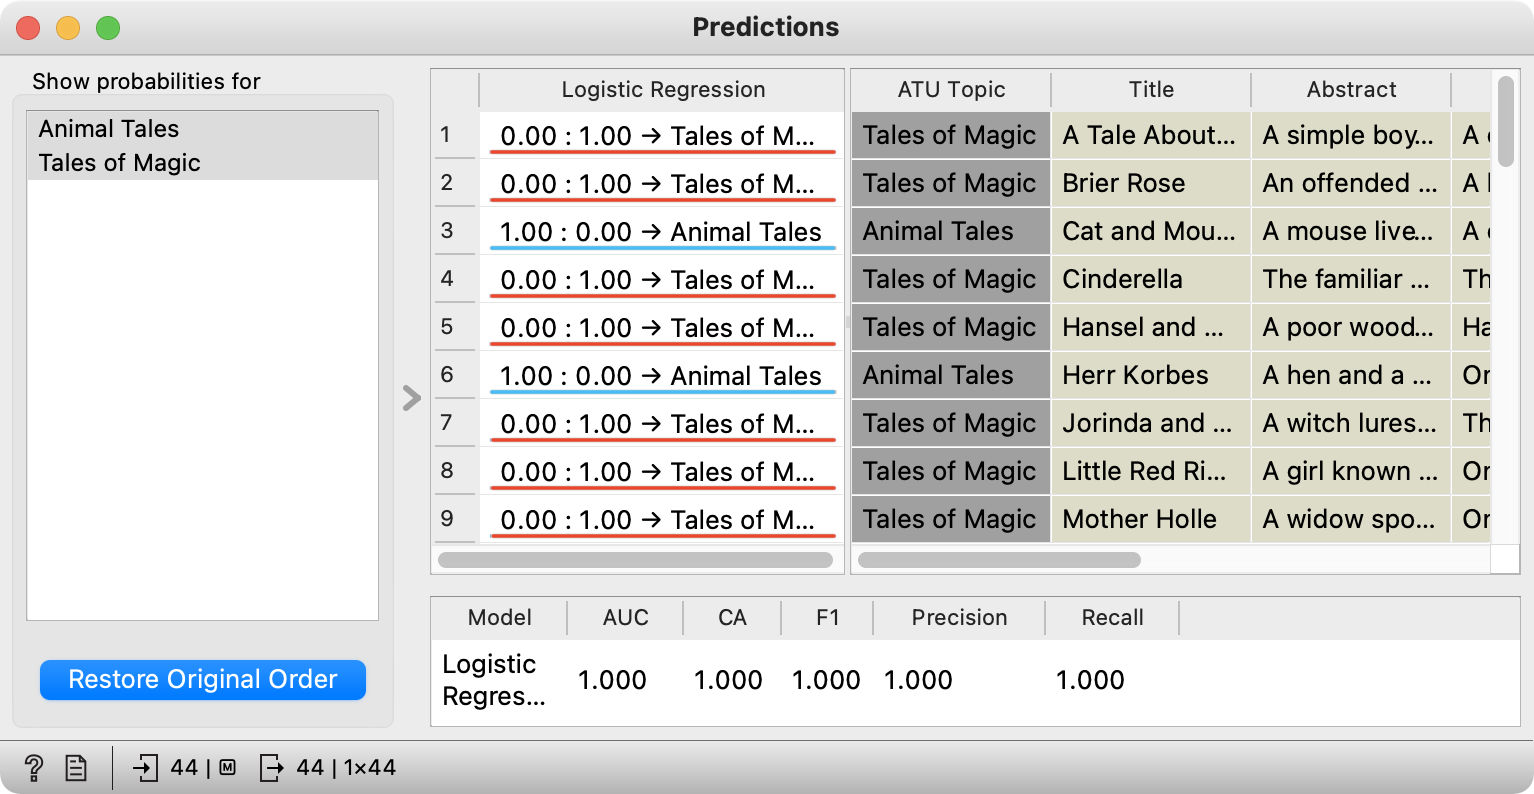
\includegraphics[width=0.95\linewidth]{predictions.png}%
    \caption{ }
    \label{fig:002-word-cloud}
\end{figure*}